\documentclass[9pt,twocolumn,twoside]{pnas-new}
% Use the lineno option to display guide line numbers if required.
% Note that the use of elements such as single-column equations
% may affect the guide line number alignment. 

\templatetype{pnasresearcharticle} % Choose template 
% {pnasresearcharticle} = Template for a two-column research article
% {pnasmathematics} = Template for a one-column mathematics article
% {pnasinvited} = Template for a PNAS invited submission

% added to enable supplementary figures
\usepackage{placeins}
\usepackage{newfloat}
\DeclareFloatingEnvironment[name={Figure}]{suppfigure}
\renewcommand{\thesuppfigure}{S\arabic{suppfigure}}

\DeclareFloatingEnvironment[name={Dataset}]{suppdata}
\renewcommand{\thesuppdata}{S\arabic{suppdata}}

\newcommand{\comment}[1]{{\color{red}[\textsl{#1}]}}

\title{Deep mutational scanning of hemagglutinin helps distinguish the evolutionary fate of human H3N2 influenza virus lineages}

% Use letters for affiliations, numbers to show equal authorship (if applicable) and to indicate the corresponding author
\author[a,d,e,1]{Juhye M. Lee}
\author[b,f,1]{John Huddleston} 
\author[a,d,e]{Michael B. Doud}
\author[a,f]{Kathryn A. Hooper}
\author[b,c,2]{Trevor Bedford}
\author[a,c,d,2]{Jesse D. Bloom}

\affil[a]{Basic Sciences Division}
\affil[b]{Vaccine and Infectious Diseases Division}
\affil[c]{and Computational Biology Program, Fred Hutchinson Cancer Research Center, Seattle, WA 98109, USA}
\affil[d]{Department of Genome Sciences}
\affil[e]{Medical Scientist Training Program}
\affil[f]{and Molecular and Cellular Biology Program, University of Washington, Seattle, WA 98195, USA}

% Please give the surname of the lead author for the running footer
\leadauthor{Lee} 

% Please add here a significance statement to explain the relevance of your work
\significancestatement{Authors must submit a 120-word maximum statement about the significance of their research paper written at a level understandable to an undergraduate educated scientist outside their field of speciality. The primary goal of the Significance Statement is to explain the relevance of the work in broad context to a broad readership. The Significance Statement appears in the paper itself and is required for all research papers.}

% Please include corresponding author, author contribution and author declaration information
\authorcontributions{Please provide details of author contributions here.}
\authordeclaration{Please declare any conflict of interest here.}
\equalauthors{\textsuperscript{1}J.M.L. and J.H. contributed equally to this work.}
\correspondingauthor{\textsuperscript{2}To whom correspondence should be addressed: trevor@bedford.io, jbloom@fredhutch.org}

% Keywords are not mandatory, but authors are strongly encouraged to provide them. If provided, please include two to five keywords, separated by the pipe symbol, e.g:
\keywords{influenza virus $|$ hemagglutinin $|$ deep mutational scanning $|$ antigenic drift $|$ epistasis} 

\begin{abstract}
Please provide an abstract of no more than 250 words in a single paragraph. Abstracts should explain to the general reader the major contributions of the article. References in the abstract must be cited in full within the abstract itself and cited in the text.
\end{abstract}

\dates{This manuscript was compiled on \today}
\doi{\url{www.pnas.org/cgi/doi/10.1073/pnas.XXXXXXXXXX}}

\begin{document}

% Optional adjustment to line up main text (after abstract) of first page with line numbers, when using both lineno and twocolumn options.
% You should only change this length when you've finalised the article contents.
\verticaladjustment{-2pt}

\maketitle
\thispagestyle{firststyle}
\ifthenelse{\boolean{shortarticle}}{\ifthenelse{\boolean{singlecolumn}}{\abscontentformatted}{\abscontent}}{}

% If your first paragraph (i.e. with the \dropcap) contains a list environment (quote, quotation, theorem, definition, enumerate, itemize...), the line after the list may have some extra indentation. If this is the case, add \parshape=0 to the end of the list environment.
\dropcap{V}ery rough outline:
\begin{itemize}
\item Mutations are rampant in the evolution of human influenza virus. Seasonal H3N2 influenza virus in particular rapidly accumulates mutations.
\item The evolution of H3N2 is also characterized by clade competition and population turnover.
\item There have been efforts to predict evolutionary success.
\item Mutations that contribute to antigenic evolution largely determine strain success.
\item RNA viruses can accumulate deleterious mutations, and because the influenza does not appreciably recombine, deleterious mutations are linked to beneficial ones.
\item Mutations in HA that impact viral growth may influence strain success.
\item We need to understand the functional impact of mutations in HA.
\item Previously, we measured the effect of all possible single amino-acid mutations to an H1 hemagglutinin from the A/WSN/1933 (H1N1) strain~\citep{thyagarajan2014inherent,doud2016accurate}. 
\item However, this is a highly lab-adapted strain, and the measurements in this strain may not be particularly relevant for studying mutational processes of more contemporaneous strains circulating in the human population.
\item We chose to study the Perth/2009 H3 HA.
\item This also enabled a comparison of how the preferences have shifted for two diverged HA's.
\end{itemize}

 

\section*{Results}
\label{sec:results}

\subsection*{Deep mutational scanning of HA from a recent strain of human H3N2 influenza virus}
We performed a deep mutational scan to measure the effects of all amino-acid mutations to HA from the A/Perth/16/2009 (H3N2) strain on viral replication in cell culture. 
This strain was the H3N2 component of the influenza vaccine from 2010-2012~\cite{who2010d,who2011}.
Relative to the consensus sequence for this HA in Genbank, we used a variant with two mutations that enhanced viral replication in cell culture, G78D and T212I (Figure~\ref{suppfig:Perth2009_mut} and Dataset~\ref{suppdata:PerthHA}).
The G78D mutation occurs at low frequency in natural H3N2 sequences, and T212 is a site where a mutation to Ala rose to fixation in human influenza in $\sim$2011.

We mutagenized the entire HA coding sequence at the codon level to create mutant plasmid libraries harboring an average of $\sim$1.4 codon mutations per clone (\comment{supplementary figure with Sanger sequencing}).
We then generated mutant virus libraries from the mutant plasmids using a helper-virus system that enables the efficient generation of complex influenza virus libraries~\cite{doud2016accurate} (Figure~\ref{fig:dms_overview}A).
These mutant viruses derived all of their non-HA genes from the lab-adapted WSN/1933 strain.
Using WSN/1933 for the non-HA genes reduces biosafety concerns, and also helped increase viral titers.
To further increase viral titers, we used MDCK-SIAT1 cells that we had engineered to constitutively express the TMPRSS2 protease, which facilitates HA cleavage and activation~\cite{bottcher2006proteolytic, bottcher2010cleavage}.

After generating the mutant virus libraries, we passaged them at low MOI in cell culture to create a genotype-phenotype link and select for functional HA variants (Figure~\ref{fig:dms_overview}A).
All of the experiments were completed in full biological triplicate (Figure~\ref{fig:dms_overview}B). 
We also passaged and deep sequenced library 3 in duplicate (denoted as library 3-1 and 3-2) to gauge to the amount of experimental noise occurring \textit{within} a single biological replicate.
As a control to measure sequencing and mutational errors, we used the unmutated HA gene to generate and passage viruses carrying wildtype HA.

Deep sequencing of the initial plasmid mutant libraries and the passaged mutant viruses allowed us to observe selection for functional HA mutants.
As expected, selection against non-functional HA variants as led to reduced mutation frequencies in the mutant viruses compared to the initial mutant plasmids (Figure~\ref{fig:dms_overview}C).
Specifically, stop codons were purged to 20-45\% of their initial frequencies after correcting for error rates estimated by sequencing the wildtype controls.
The incomplete purging of stop codons is likely because genetic complementation due to co-infection \comment{let's cite some paper here, maybe Chris Brooke one?} enabled the persistence of some virions with nonfunctional HAs. 
We also observed selection against many nonsynonymous mutations, with their frequencies falling to 30-40\% of their initial values after error correction.

\begin{figure*}
\centering
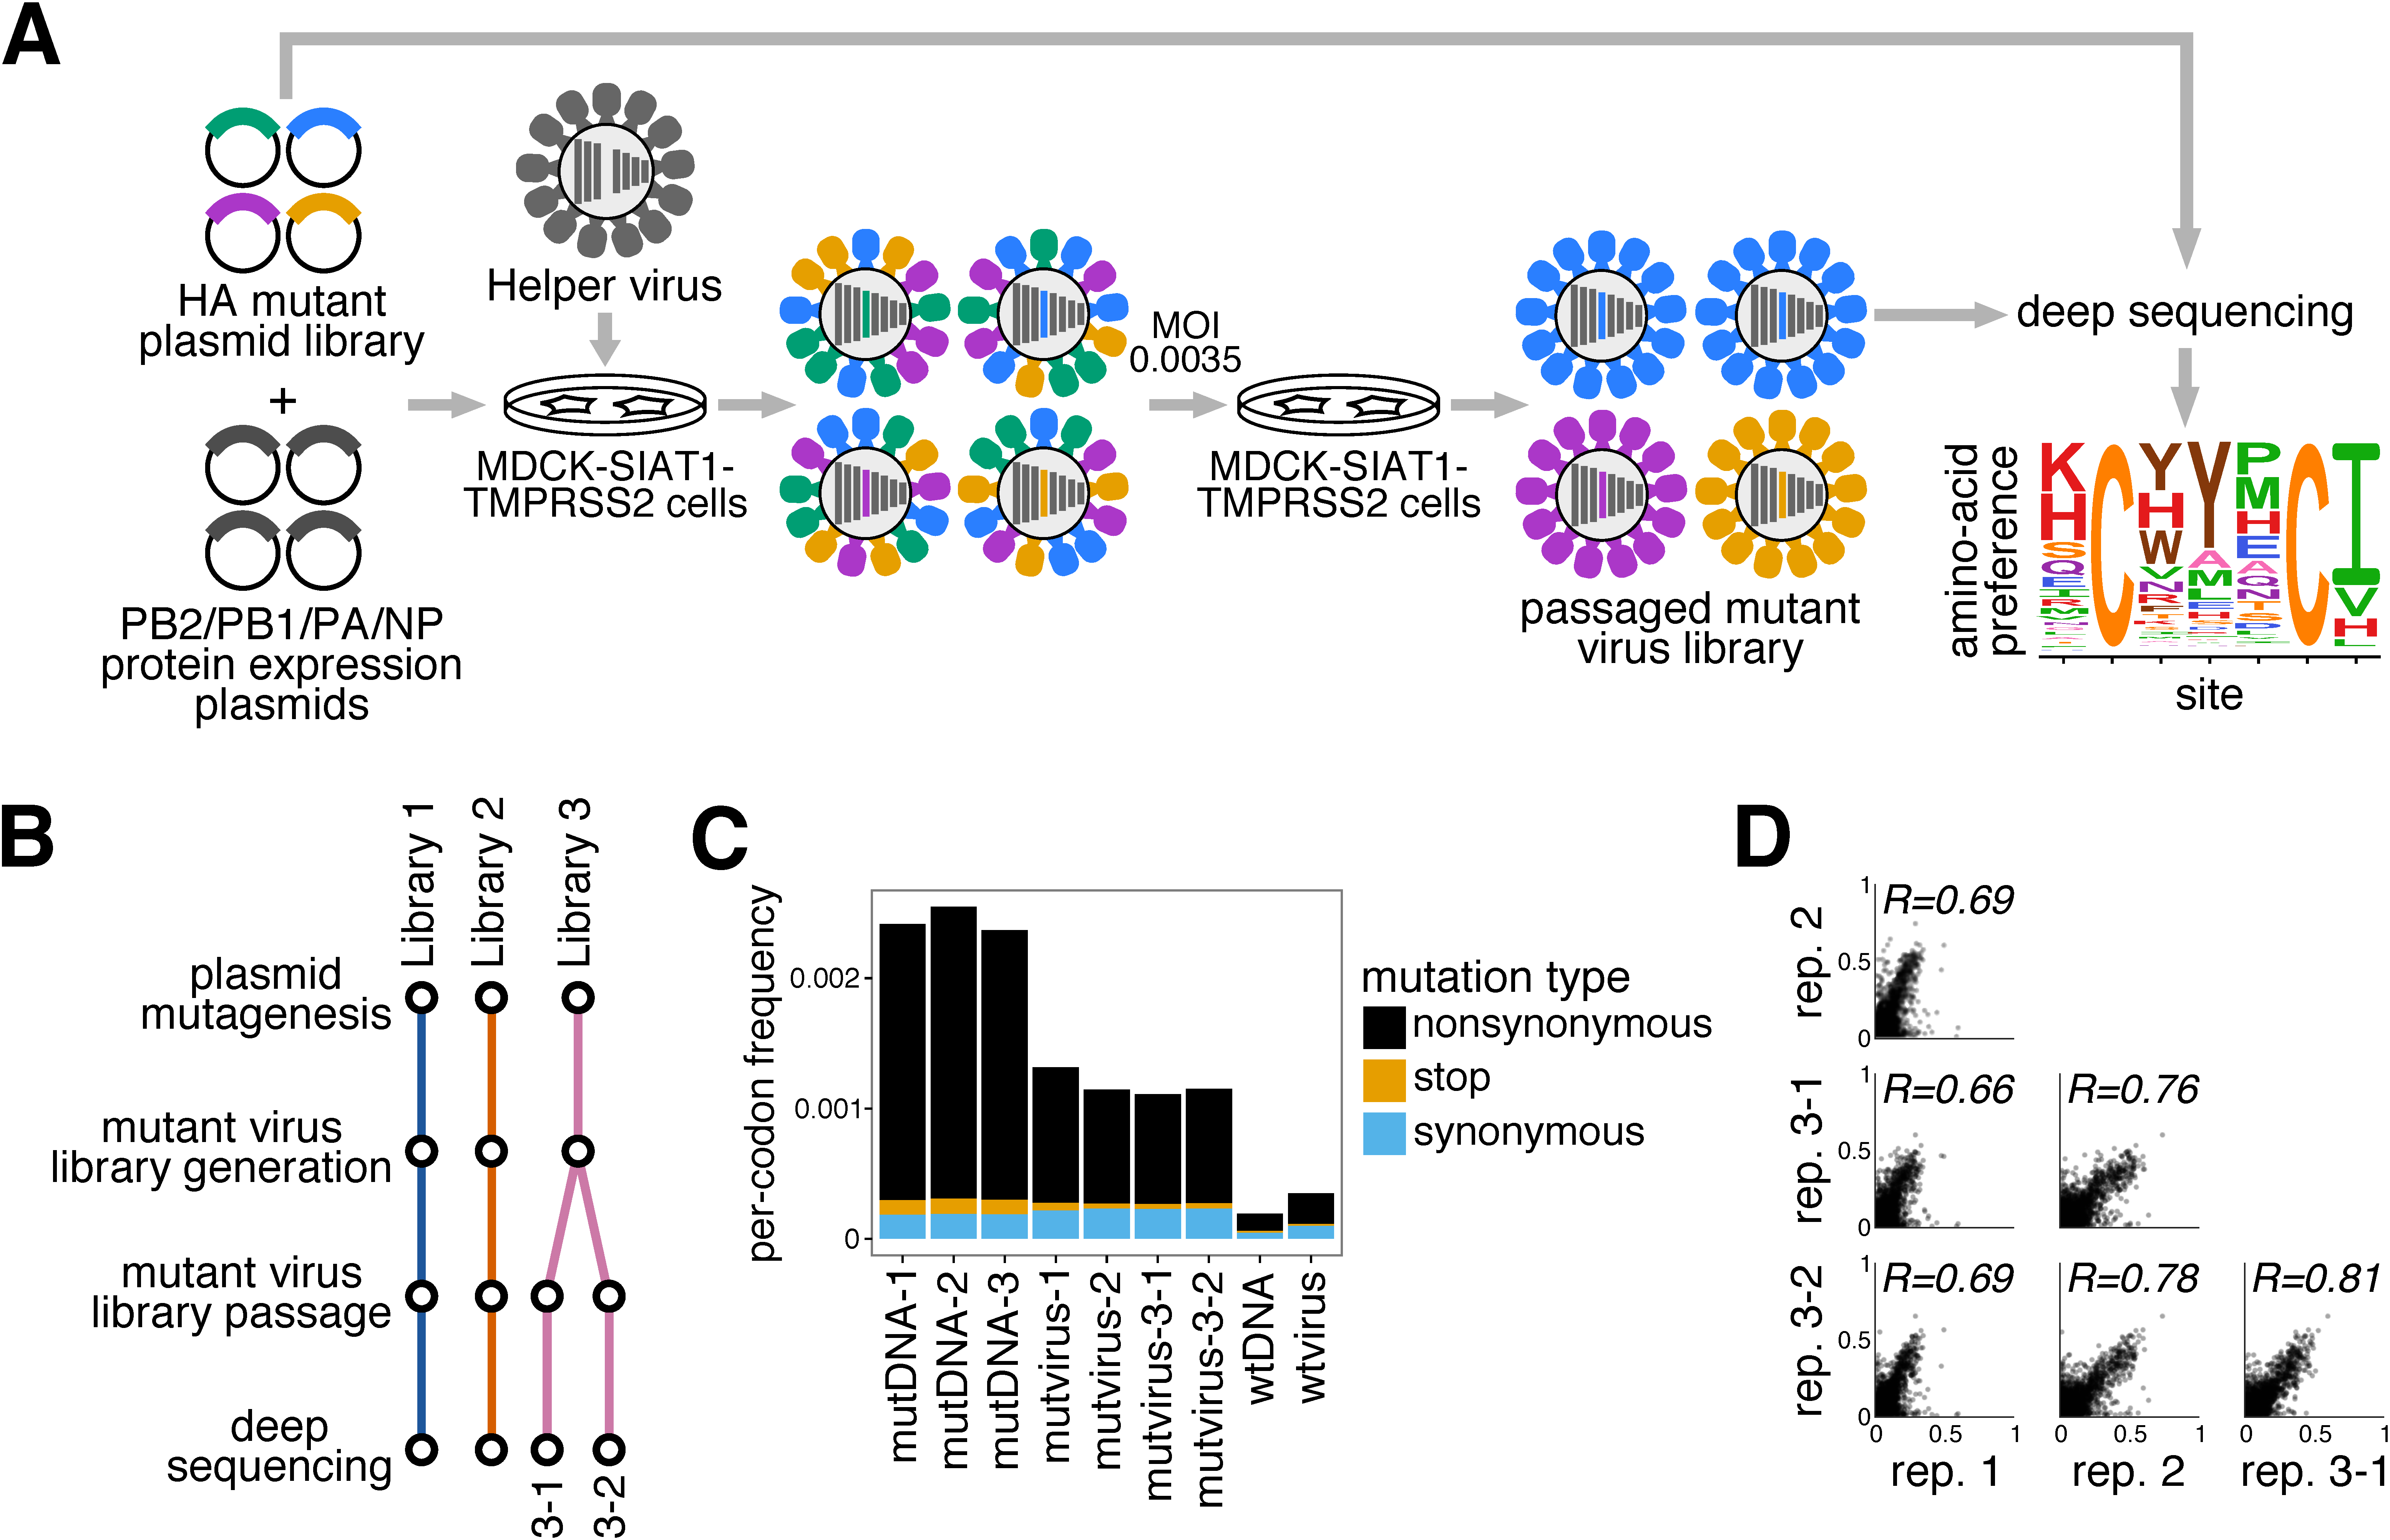
\includegraphics[width=13cm]{figs/dms_overview/dms_overview.pdf}
\caption{\label{fig:dms_overview}
{\bf Deep mutational scanning of the Perth/2009 H3 HA.}
(A) We generated mutant virus libraries using a helper-virus approach~\cite{doud2016accurate}, and passaged them at low MOI to establish a genotype-phenotype linkage and to select for functional HA variants. 
Deep sequencing of the variants before and after selection allowed us to estimate each site's amino-acid preferences.
(B) The experiments were performed in full biological triplicate. 
We also passaged and deep sequenced library 3 in duplicate.
(C) Frequencies of nonsynonymous, stop, and synonymous mutations in the mutant plasmid DNA, the passaged mutant viruses, and wildtype DNA and virus controls. 
(D) The Pearson correlations among the amino-acid preferences estimated in each replicate. 
}
\end{figure*}

We next quantified the reproducibility of our deep mutational scanning measurements across biological and technical replicates. 
We first used the deep sequencing data for each replicate to independently estimate the preference of each site in HA for all 20 amino acids using the method described in~\cite{bloom2015software}.
Because there are 567 residues in HA, there are $567 \times 20 = 11,340$ estimated amino-acid preferences.
The correlations of the amino-acid preferences between pairs of replicates are shown in Figure~\ref{fig:dms_overview}D.
The biological replicates are fairly well-correlated, with Pearson's $R$ ranging from 0.69 to 0.78. 
Replicate 1 exhibited the lowest correlation with the other replicates, consistent with the observation that this replicate also showed the weakest selection against stop and nonsynonymous mutations perhaps indicating more experimental noise.
The two technical replicates 3-1 and 3-2 were only slightly more correlated than pairs of biological replicates, suggesting that bottlenecking of library diversity after the reverse-genetics step contributes most of the experimental noise.

\subsection*{Our measurements are consistent with existing knowledge about HA's evolution and function}
How do the HA amino-acid preferences measured in our experiments relate to the evolution of H3N2 influenza virus in nature?
This question can be addressed by evaluating how well an experimentally informed codon substitution model (ExpCM) using our measurements describe H3N2 evolution compared to standard phylogenetic substitution models~\cite{hilton2017phydms}.
Table~\ref{tab:phydms} shows that the ExpCM greatly outperforms conventional substitution models, showing that our experiments authentically capture some of the constraints on HA evolution. 
\comment{Jesse and Juhye are here in sentence-level editing} 
The ExpCM also optimizes a stringency parameter for the preferences to more closely reflect the strength of selection in nature.
The stringency parameter in the ExpCM is equal to 2.44, which indicates that although the same amino acids are preferred, the strength of selection is more stringent in nature than in our experiments.
Figure~\ref{fig:logoplot} shows a logo plot of the Perth/2009 HA amino-acid preferences rescaled by this stringency parameter.

\begin{figure*}
\centering
\caption{\label{tab:phydms}
{\bf The site-specific amino-acid preferences are informative for describing human H3N2 evolution in nature.}}
\begin{tabular}{cccccccc}
\hline
\bf{Model} & \bf{$\Delta$AIC} & \bf{Log Likelihood} & \bf{Stringency} & \bf{$\omega$} & \bf{$\overline{\omega}$} & \bf{$\omega_{\alpha}$} & \bf{$\omega_{\beta}$} \\ \hline
ExpCM & 0.0 & -8439.33 & $2.44$ & $0.91$ & -- & -- & -- \\
Goldman-Yang M5 & 2166.06 & -9516.36 & -- & -- & $0.36$ & $0.30$ & $0.84$ \\
ExpCM, averaged across sites & 2504.18 & -9691.42 & $0.68$ & $0.32$ & -- & -- & -- \\
Goldman-Yang M0 & 2607.92 & -9738.29 & -- & $0.31$ & -- & -- & -- \\
\hline
\end{tabular}

\addtabletext{We implemented several codon substitution models for phylogenetic fitting of an alignment of human H3N2 HA sequences. 
The maximum likelihood values for each model were compared using the Akaike information criteria ($\Delta$AIC)~\cite{posada2004model}.
An experimentally-informed codon substitution model (ExpCM) built from the preferences averaged across all replicates performs better than conventional substitution models, specifically the M0 and M5 models in~\cite{yang2000codon}.
A non-site-specific ExpCM informed by preferences averaged across all sites performs comparably to the GY94 class of models, indicating the importance of site-specificity in the ExpCM.
The optimized parameters for each model are also shown.}
\end{figure*}

A closer examination of the logo plot reveals that the preferences generally agree with existing knowledge about HA's biochemistry.
For instance, sites that form structurally important disulfide bridges (sites 52 \& 277, 64 \& 76, 97 \& 139, 281 \& 305, 14 \& 137-HA2, 144-HA2 \& 148-HA2)~\cite{waterfield1981disulphide} possess high preference for cysteine.
At residues involved in receptor binding, there are strong preferences for the amino acids at sites Y98, D190, W153, and S228~\cite{weis1988structure,martin1998studies}.
A positively charged amino acid at site 329 is important for cleavage activation of the HA0 precursor, and indeed this site exhibits a high preference for arginine~\cite{kido1992isolation, stech2005new}.
However, a notable exception occurs at the start codon at position -16, which does not show a strong preference for methionine. 
This codon is part of the signal peptide and is cleaved from the mature HA protein.
One possible explanation for why we do not see a strong preference for Met at this site is due to alternative translation initiation occurring at a downstream or upstream start site, as has been described for HA~\cite{girard2011upstream}.
% No upstream or downstream "ATG"'s are present. I did find an in-frame "ATC" one codon upstream of the canonical start site (in the non-coding region), and interestingly, all Perth/2009 HA sequences deposited in GenBank have an "ATT" in this non-coding position, including Seema's Perth HA.
% I6M(HA2) mutant slightly increases the fusion pH (Daniels 1985 Cell)
% We see high preference for T,S,Q over the wildtype Ile at site 226. Although Q226 in an H3 background is characterized as having preference for avian-type receptors, most of these studies were done in older H3 strains such as Aichi. Wu 2017 Cell Host Microbe has shown extensive epistasis in the RBS, specifically in the 220-loop, so perhaps the amino acids tolerated in this loop have shifted over time. Indeed the wildtype amino acids at 225 and 226 are different in Perth compared to HK68 and Aichi.

\begin{figure*}
\centering
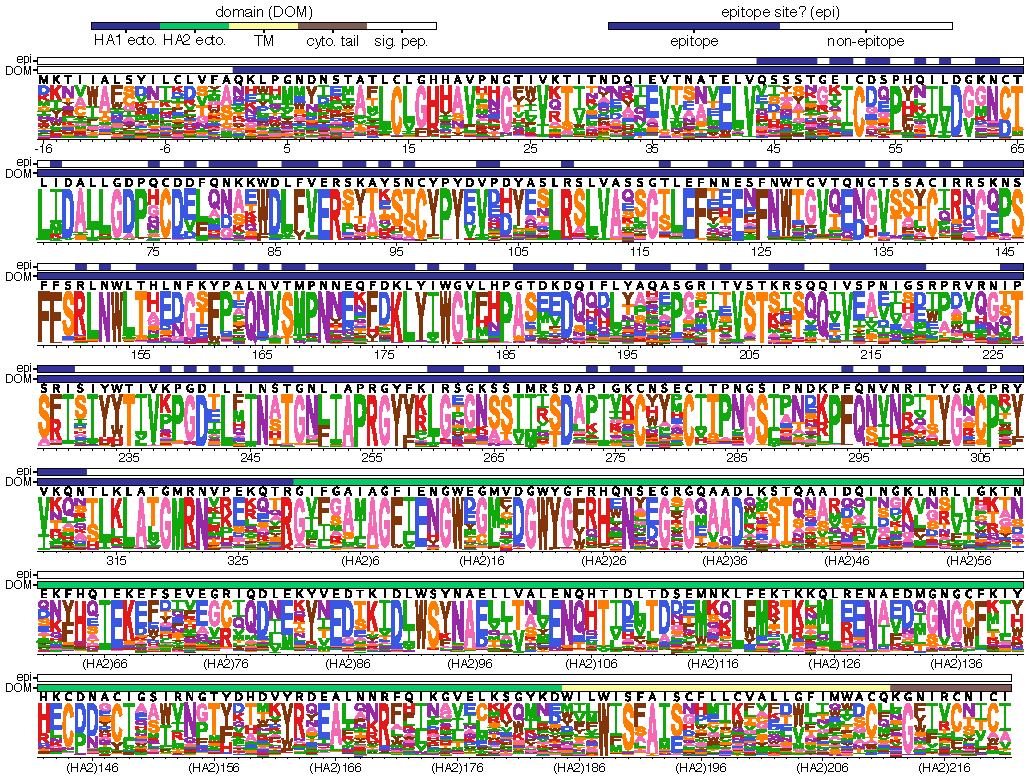
\includegraphics[width=17cm]{figs/prefslogoplot/rescaled-avgprefs_prefs.pdf}
\caption{\label{fig:logoplot}
{\bf The site-specific amino-acid preferences of the Perth/2009 HA.}
This logoplot shows the site-specific amino-acid preferences for the averaged replicates rescaled by the stringency parameter (Table 1) estimated by phydms.
The height of each letter is proportional to its preference at that site, and the preferences for all sites are normalized to sum to 1.
The sites are in H3 numbering.
The top overlay bar shows the relative solvent accessibility.
The bottom overlay bar is colored by the HA domain (sig. pep. = signal peptide, HA1 ecto. = HA1 ectodomain, HA2 ecto. = HA2 ectodomain, TM = transmembrane domain, cyto. tail. = cytoplasmic tail).
The letters directly above each logo indicate the wildtype amino acid at that site.
}
\end{figure*}

\subsection*{The mutational tolerance of the head and the stalk shows less of a contrast in H3 than in H1}
We next sought to investigate the inherent mutational tolerance of the Perth/2009 HA. 
Figure~\ref{fig:mut_tolerance} shows the mutational tolerance as calculated from the rescaled Perth/2009 H3 preferences and the rescaled WSN/1933 H1 preferences mapped onto the HA crystal structures.
We found antigenic site C and the most distal portion of the globular head near the 190-helix in the Perth/2009 H3 to be tolerant of mutations.
Interestingly, the H3 stalk including the shorter $\alpha$-helix (helix A) is relatively mutationally tolerant compared to the tolerance of the globular head domain. 
This observation suggests that the stalk may be prone to escape from antibodies, and agrees with previous work demonstrating that it is possible to select for antigenic mutants in H3 by broadly-neutralizing stalk-targeting antibodies~\cite{ekiert2011highly, friesen2014common, chai2016two, yamayoshi2017human}.
% In contrast, the head domain of the WSN/1933 H1 is more mutationally tolerant relative to its stalk domain.

The sites inside the receptor binding pockets are highly functionally constrained and were found to be relatively mutationally intolerant in both H3 and H1~\citep{wilson1981structure}.
In contrast, the residues surrounding the receptor binding pocket are fairly mutationally tolerant, which may contribute to antigenic evolution as these sites are under strong immune pressure.~\citep{wiley1981structural}.

\begin{figure*}
\centering
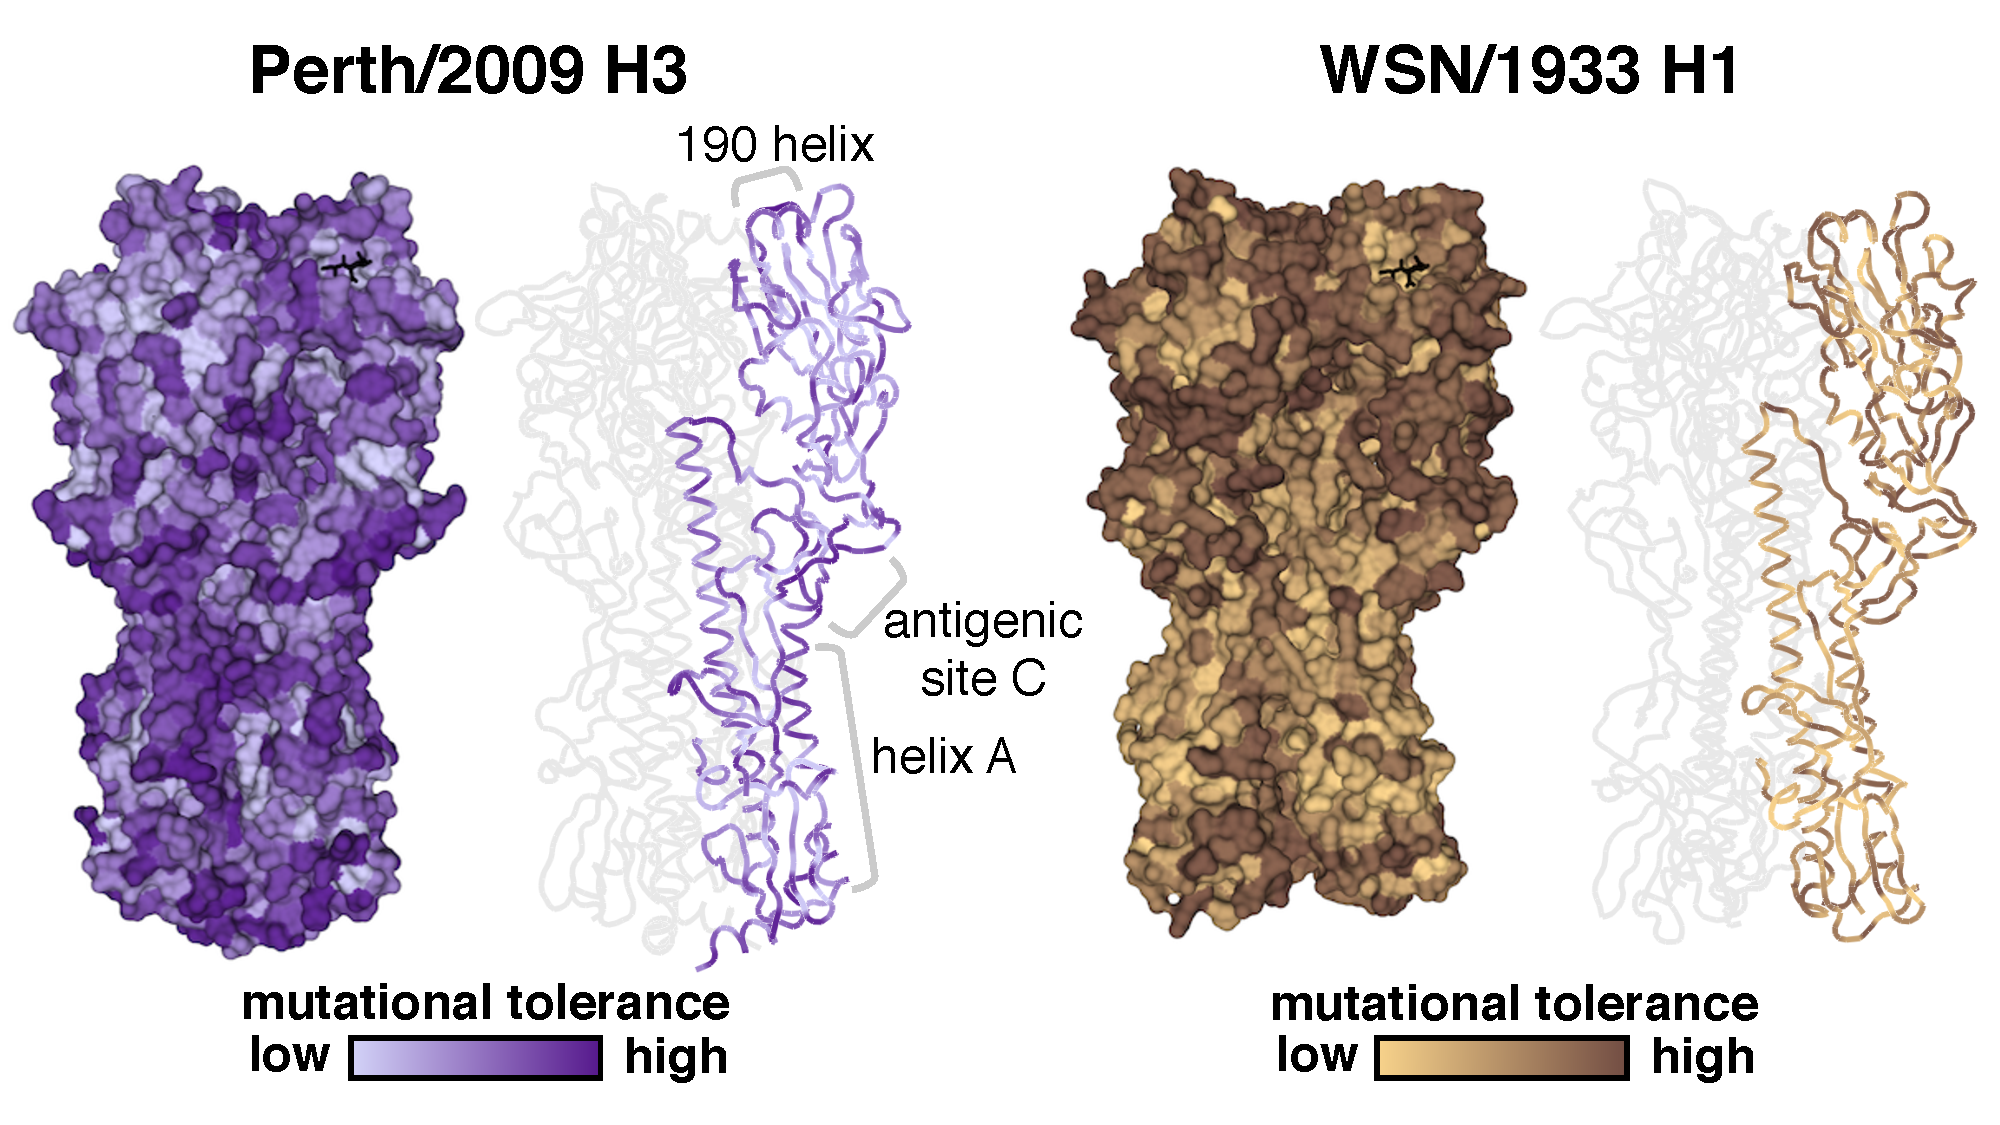
\includegraphics[width=16cm]{figs/mut_tolerance/entropy_heatmap.pdf}
\caption{\label{fig:mut_tolerance}
{\bf Mutational tolerance mapped onto each site of HA.}
Mutational tolerance as calculated by the Shannon entropy of a given site's amino-acid preferences are mapped onto the structure of the H3 trimer (PDB 4O5N;~\cite{lee2014receptor}) and the H1 trimer (PDB 1RVX;~\cite{gamblin2004structure}), with both trimers in approximately the same orientation. 
The site entropies were calculated from the preferences measured in the Perth/2009 H3 (left panel) from this study, or the preferences measured in the WSN/1933 H1 (right panel) from~\cite{doud2016accurate}. 
Lighter shades of purple or brown signify low mutational tolerance, while darker shades signify high mutational tolerance. 
For each HA, the structure on the left side colors the full HA trimer, while the structure on the right side colors only one of the monomers.
The sialic acid receptor is shown as black sticks.
The Perth/2009 H3 shows relatively high mutational tolerance in the stalk region, particularly in helix A, compared to the head region. 
High mutational tolerance in H3 was also observed near antigenic site C and near the 190 helix.
The head region of the WSN/1933 H1 is mutationally tolerant compared to the relatively intolerant stalk region. 
}
\end{figure*}

\subsection*{The experimental measurements can help discriminate successful influenza virus lineages}
A challenge in vaccine strain selection is predicting which strain will dominate the upcoming influenza season.
An important question to thereby address is if our experimental measurements are useful in differentiating between strains of human H3N2 influenza virus that have succeeded and those that have died out.
To investigate this, we used our preference dataset and an H3N2 phylogeny from 1968-2012 (Figure~\ref{fig:trunkvssidebranch}A) to calculate the effects of mutations for the evolutionarily successful trunk lineage and for side branches which have died out.
We found that strains with mutations measured to be more beneficial to viral growth in our experiments tend to succeed in nature.
Figure~\ref{fig:trunkvssidebranch}B shows the effects of trunk and side branch mutations in five-year intervals for every year from 1968-2012. 
On average, trunk mutations are towards more preferred amino acids compared to side branch mutations, and this was true for all intervals.
Importantly, trunk mutations are significantly more favorable than side branch mutations when calculating the effects from the entirety of the phylogenetic tree (Figure~\ref{fig:trunkvssidebranch}C).

Because tip nodes can contain egg- or cell-passaged isolates~\citep{wu2017structural,mcwhite2016sequence,skowronski2016mutations} and our experiments were performed in cell culture, we examined the effects of mutations on terminal side branch nodes to see if these would rank more highly than internal node mutations.
Instead, terminal node mutations are on average towards less preferred amino acids than internal node mutations (Figure~\ref{fig:trunkvssidebranch}C), and both internal and terminal node mutations are significantly less favorable than those on the trunk.
Therefore, strains that have accumulated mutations that we experimentally measured to be unpreferred generally die out in nature, while more favored mutations provide a selective advantage to the trunk.
These findings demonstrate the importance of the functional impacts of HA mutations in determining strain success.

\begin{figure*}
\centering
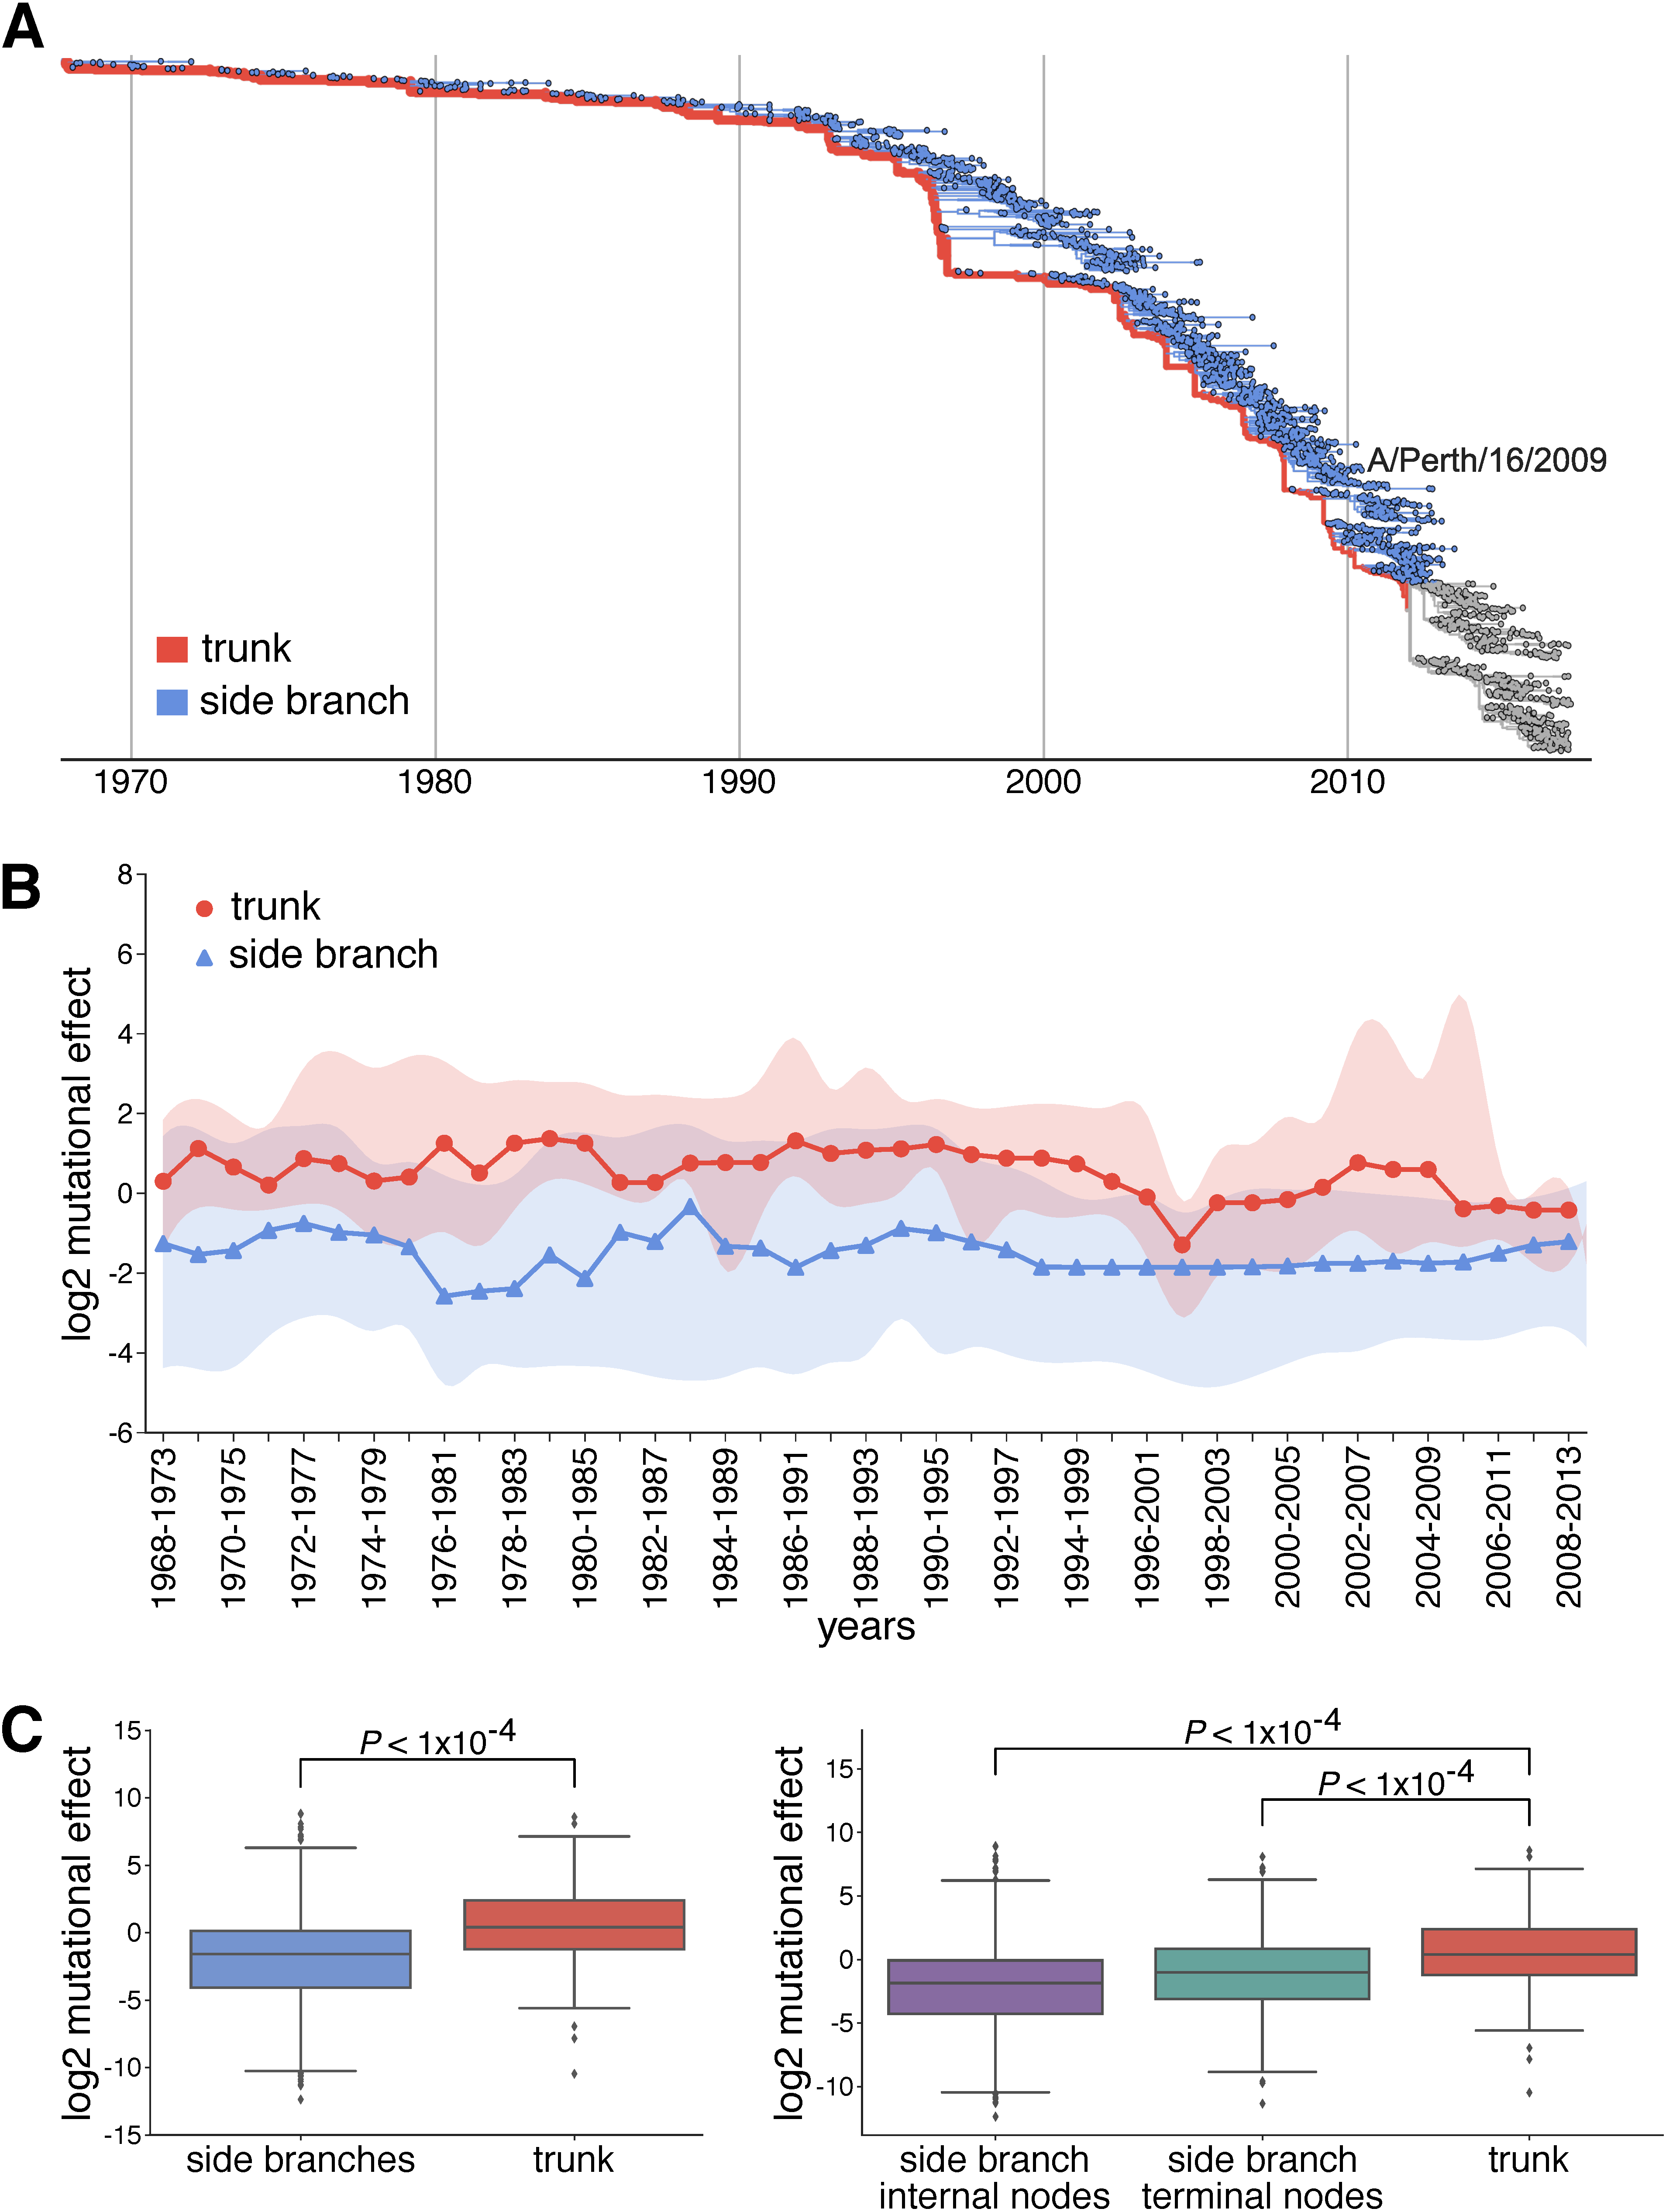
\includegraphics[width=12cm]{figs/trunkvssidebranch/trunkvssidebranch.pdf}
\caption{\label{fig:trunkvssidebranch}
{\bf Mutations in evolutionary successful strains tend to be more favorable than in strains that die out.}
(A) Phylogenetic tree of human H3N2 influenza virus from 1968-present. 
The trunk is shown in red, and side branches are shown in blue.
The gray branches represent the part of the tree for which we cannot yet distinguish the trunk from side branches.
(B) Using the Perth/2009 H3 preferences, we calculated the log$_{2}$ mutational effect for trunk and side branch mutations in windows of 5 years for every year from 1968-2013. 
The median log$_{2}$ mutational effect in a given window is shown as circles for trunk mutations and triangles for side branch mutations. 
The shaded region demarcates the interquartile range of trunk and side branch mutational effects.
Negative numbers signify mutations towards less preferred amino acids, while positive numbers signify more preferred mutations.
The median trunk mutational effects are consistently higher than the median side branch mutational effects for all windows.
(C) The log$_{2}$ mutational effect for all side branch and all trunk mutations (left panel), in addition to all mutations in internal nodes and terminal nodes on the side branches (right panel) are shown.
The preferences were randomized 10,000 times to estimate significance.
The effects of trunk mutations are higher than side branch internal and terminal node mutations.
}
\end{figure*}

How distantly can the preferences be extended to describe differences in successful and unsuccessful strains?
To explore this question, we scored the complete HA sequence of every node in the tree using the preferences by quantifying a \textit{sequence preference} metric.
The sequence preference is defined as 
$\displaystyle\sum_{r} \ln \pi_{r, a}$
where $\pi_{r, a}$ is the preference for amino acid $a$ at site $r$.
Consistent with the finding that trunk mutations are generally more favorable than side branch mutations, Figure~\ref{fig:sequence_preference} shows that the sequences of trunk nodes also tend to be more highly preferred than those of side branch nodes.
Interestingly, the sequence preferences increase over time as the nodes approach the Perth/2009 strain and its closely related nodes, which all exhibit sequence preferences that are higher than that of the trunk. 
The observation that the strain in which we performed our deep mutational scan has one of the highest sequence preferences illustrates epistatic interactions among mutations such that an unpreferred mutation in one background may be preferred in another.
% Due to the sheer number of possible pairwise combinations of mutations, it is impossible for us to experimentally characterize these epistatic interactions among mutations. 

\comment{this section will be fleshed out more once I figure out how to plot the substitutions from the root at epitope / non-epitope sites, as per Trevor's suggestion.}
We reasoned that much of the increase in sequence preference toward Perth/2009 could be attributed to epitope sites, as most substitutions have occurred at sites under strong immune pressure.
We therefore assessed each node's preference at epitope and non-epitope sites as defined by~\cite{wolf2006long}.
Indeed, the preferences at epitope sites resembles those for all HA sites (Figure~\ref{fig:sequence_preference}), with preferences increasing over time.
At non-epitope sites, however, the trunk preferences remain relatively constant while side branch preferences tend to drop below the trunk.
These observations highlight the extensive epistasis among epitope sites, as has even been noted for sites within the 220-loop surrounding the receptor binding pocket~\citep{wu2017diversity}.
Many successful epitope mutations are likely contingent upon the background in which they arise.
Yet, we are able to distinguish trunk sequences as more favorable than side branch sequences, indicating that the preferences are still of utility over short evolutionary timescales. 

\begin{figure*}
\centering
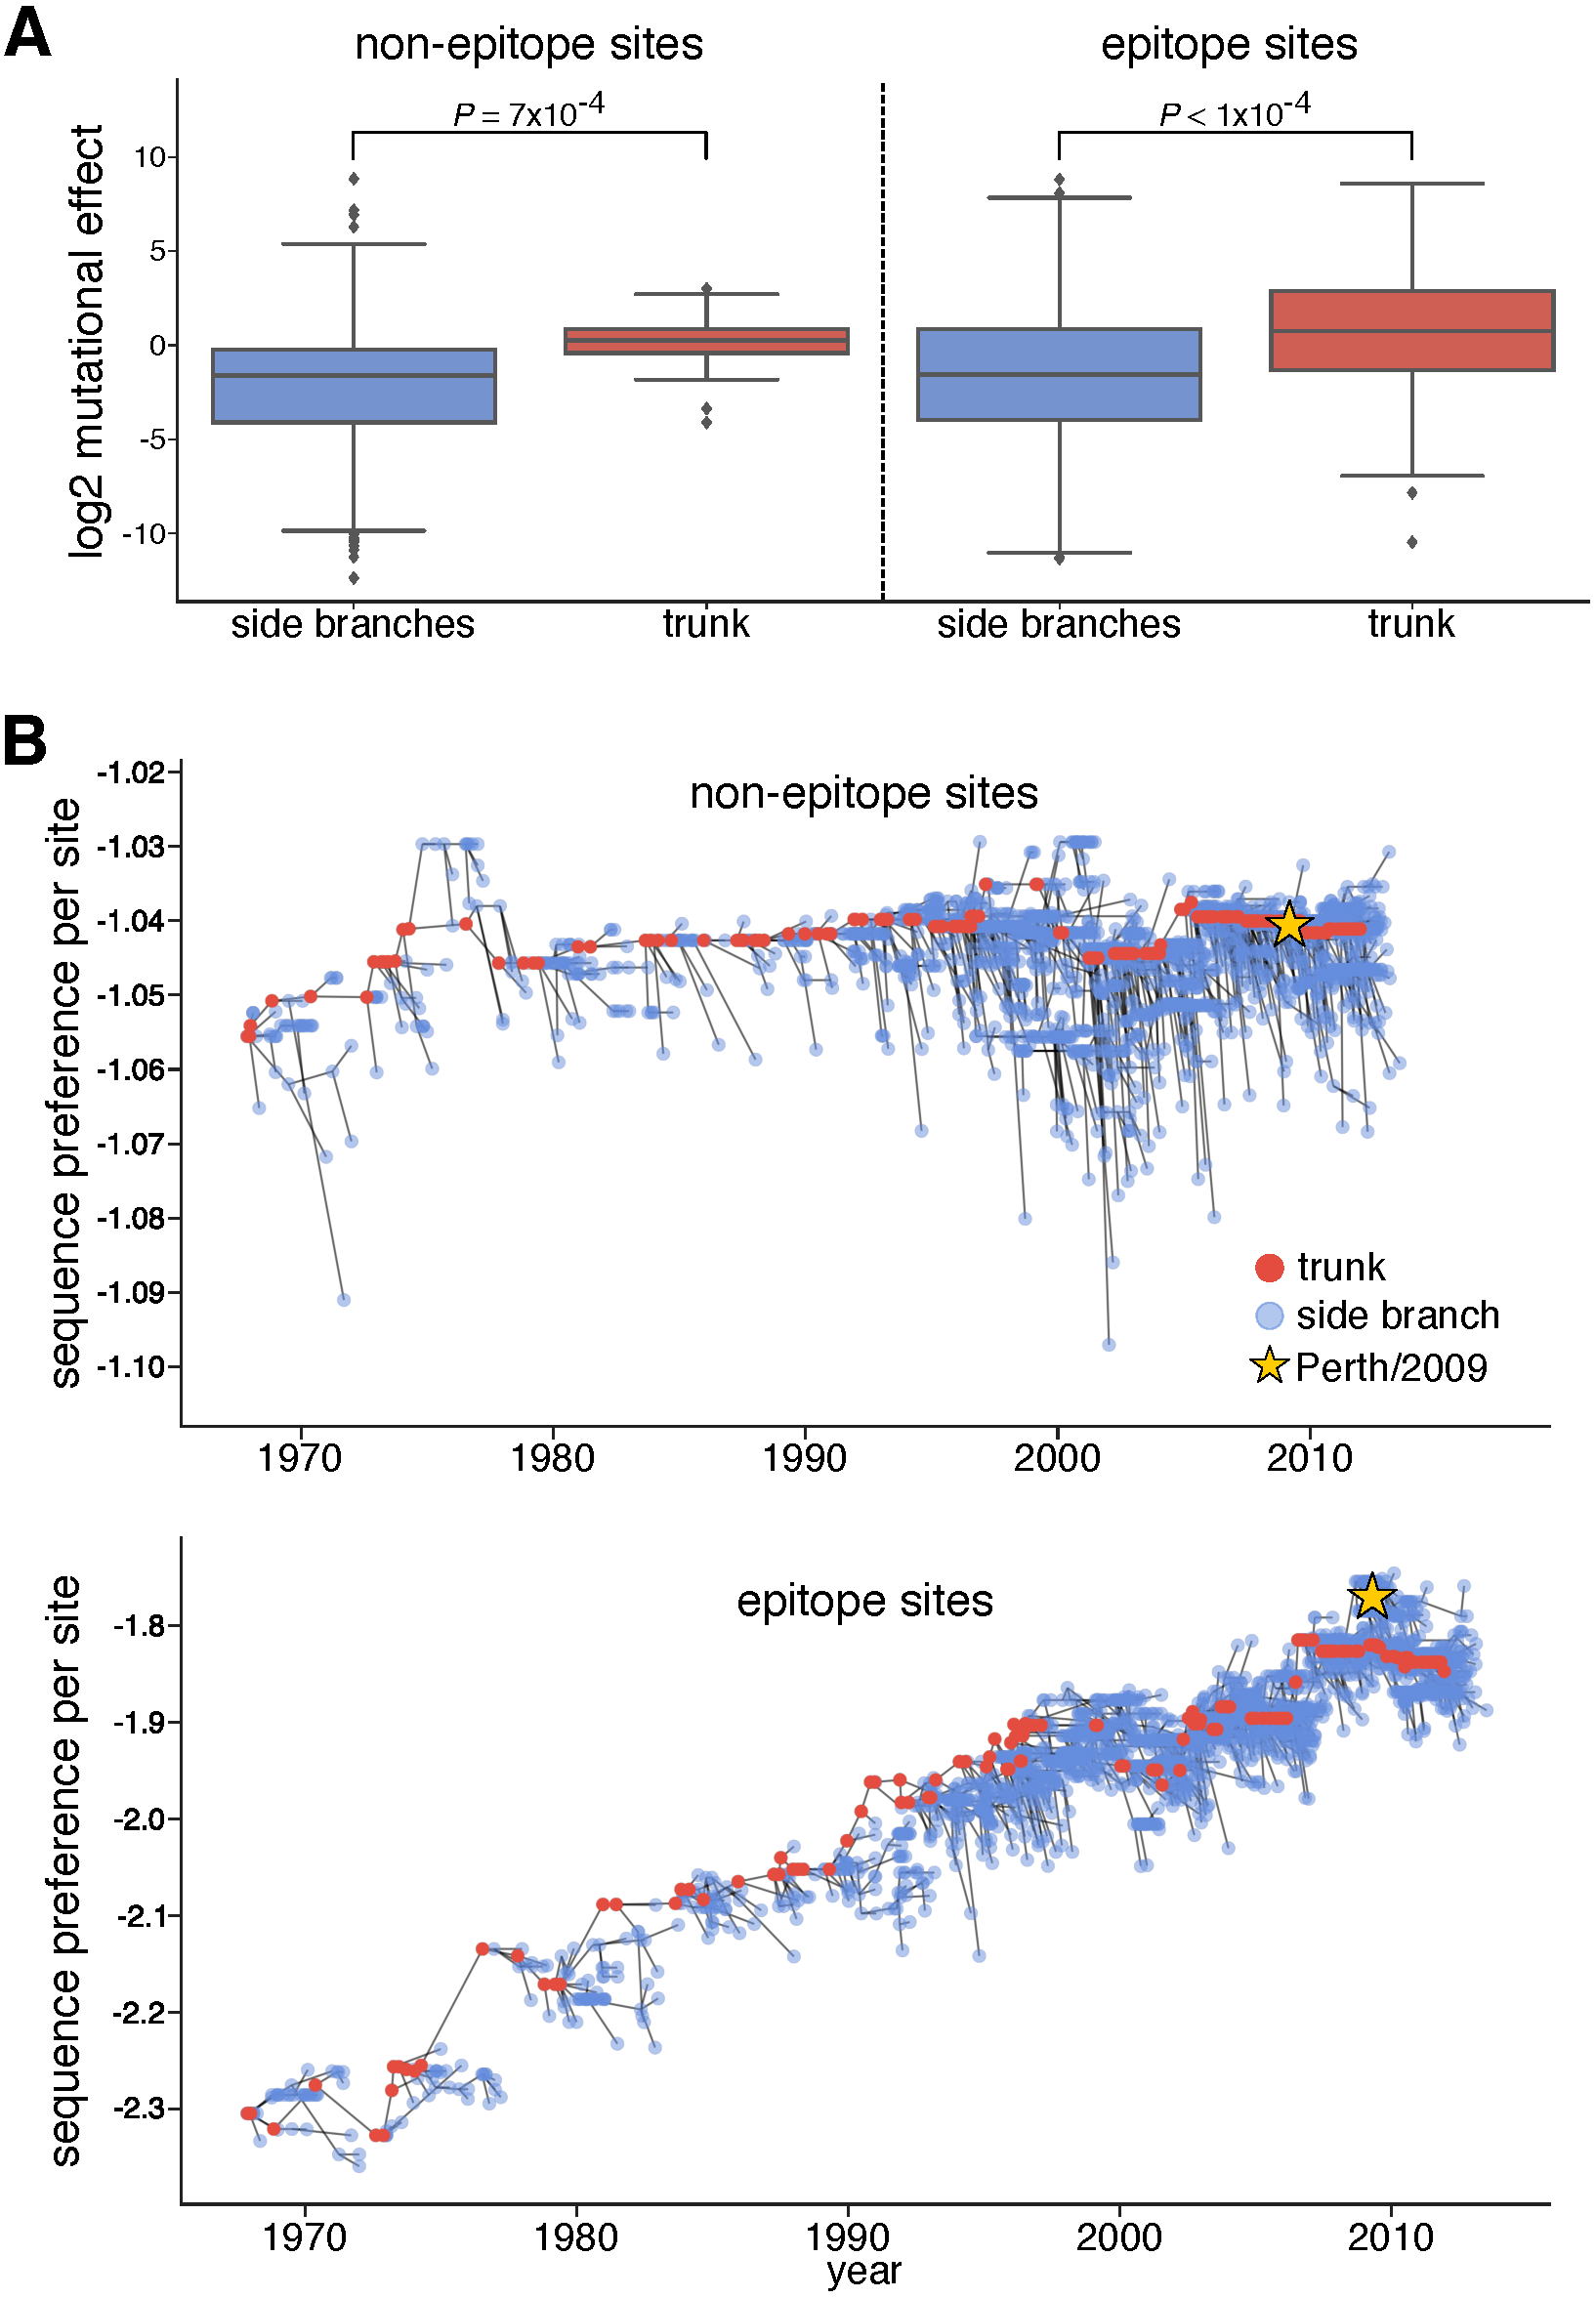
\includegraphics[width=12cm]{figs/sequence_preference/sequence_preference.pdf}
\caption{\label{fig:sequence_preference}
{\bf The HA sequences of trunk nodes tend to be more preferred than those of side branch nodes.}
We used the preferences to calculate the HA sequence preference normalized by the number of sites of every node in a human H3N2 phylogenetic tree.
To calculate the sequence preference, we used the entire HA sequence (top panel), only epitope sites (center panel) or non-epitope sites (bottom panel) as defined by~\cite{wolf2006long}.
Higher preferences are closer to zero while lower preferences are more negative.
The preferences at all sites and at epitope sites increase as the tree approaches the Perth/2009 strain, indicating epistasis among epitope sites.
The trunk nodes generally exhibit higher sequence preferences than do side branch nodes.
}
\end{figure*}

Can we then distinguish lineage-specific mutational effects using the preferences measured in a distantly related HA homolog?
We used the preferences measured previously in the WSN/1933 H1~\citep{doud2016accurate} to quantify the effects of H3 trunk and side branch mutations, shown in Figure~\ref{fig:WSN_trunkvssidebranch}.
It is evident that we do not see trunk mutations significantly more favored than side branch mutations, suggesting that our ability to discriminate successful and unsuccessful strains degrades over sufficiently long evolutionary distances. 

\begin{figure*}
\centering
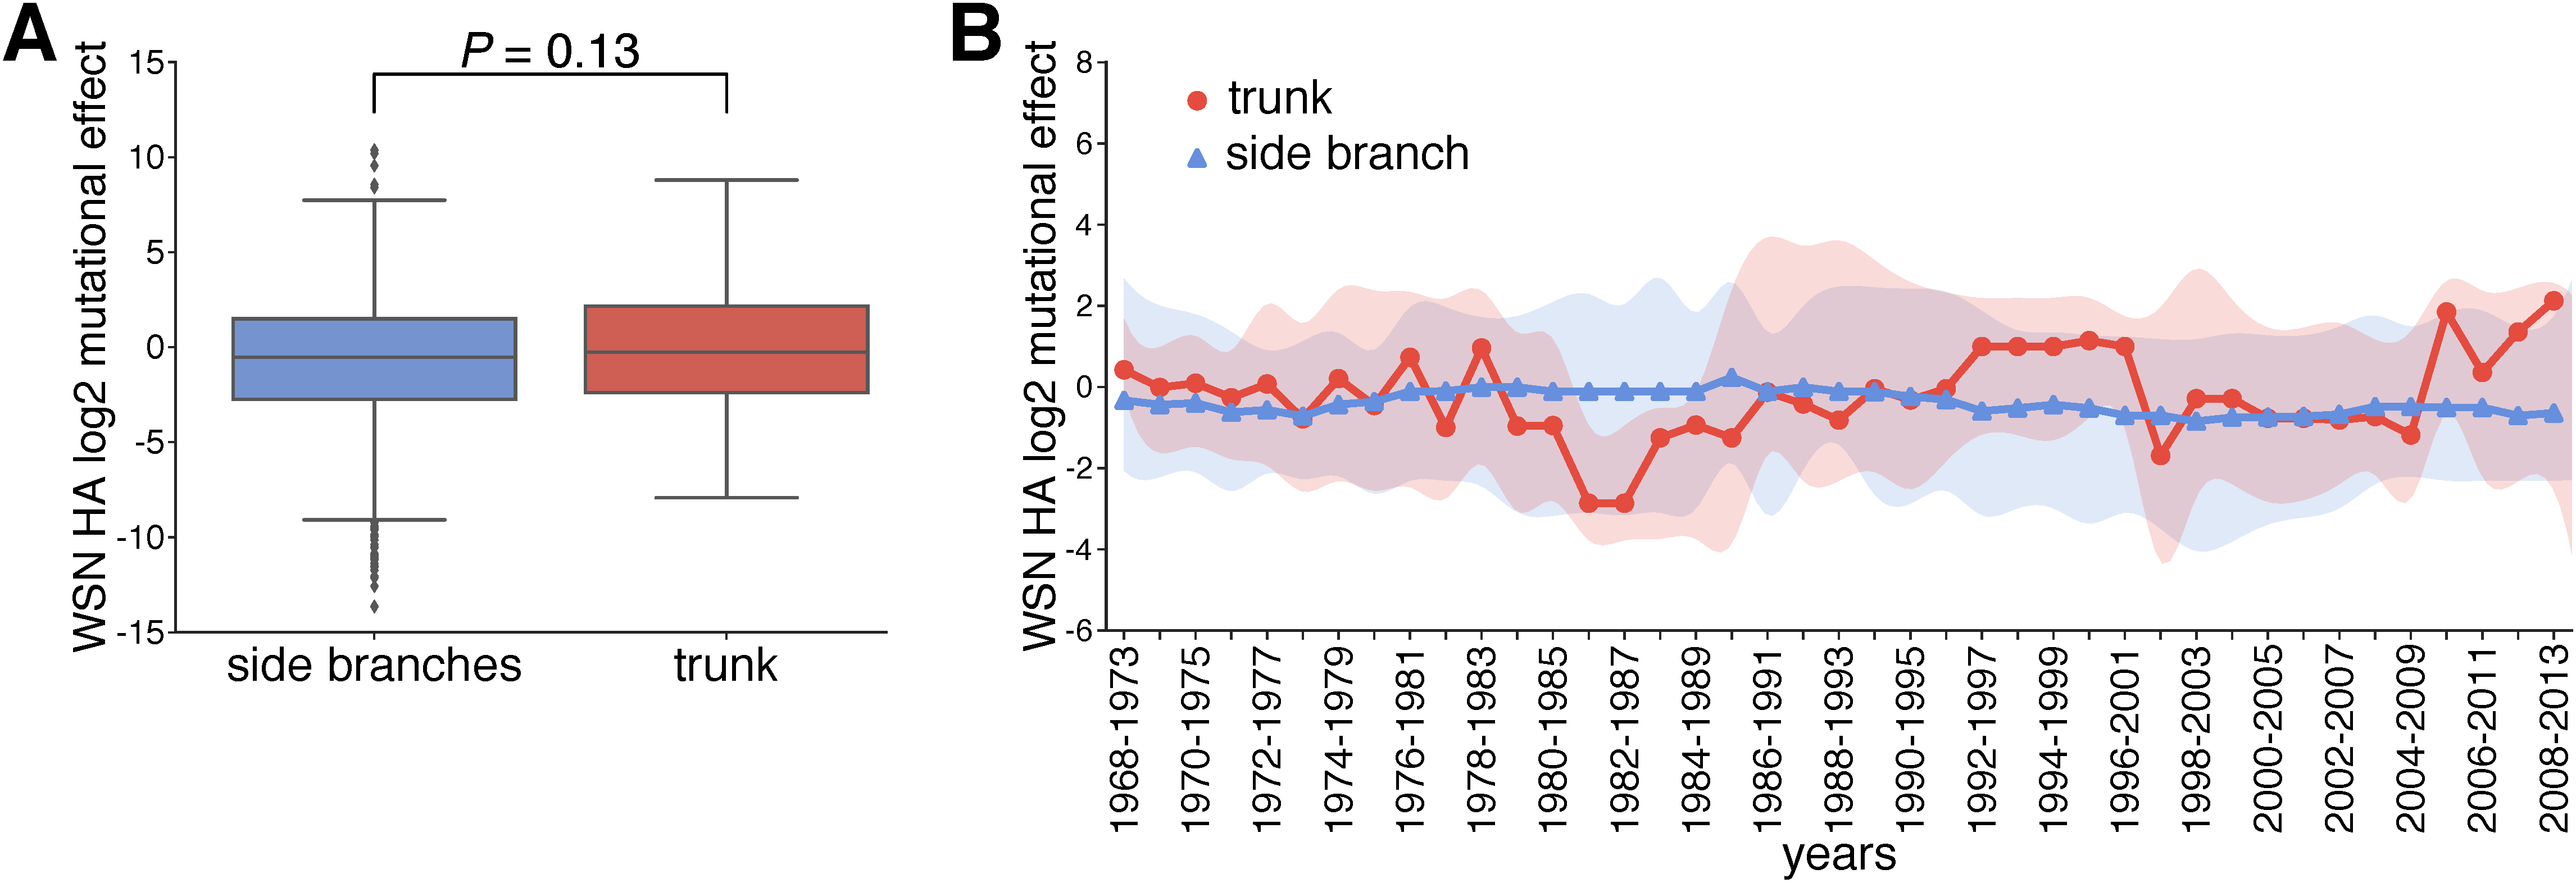
\includegraphics[width=15cm]{figs/WSN_trunkvssidebranch/WSN_trunkvssidebranch.pdf}
\caption{\label{fig:WSN_trunkvssidebranch}
{\bf The WSN/1933 H1 preferences do not reveal differences in trunk vs side branch mutational effects}
(A) We used the WSN/1933 H1 preferences from~\cite{doud2016accurate} to calculate the log$_{2}$ mutational effects of trunk and side branch mutations from the inferred H3N2 phylogeny in Figure~\ref{fig:trunkvssidebranch}.
There is not a significant difference in trunk vs side branch mutational effects.
(B) We also performed a sliding window analysis with the WSN/1933 H1 preferences.
There is not a distinct difference in trunk and side branch mutational effects.
}
\end{figure*}

\subsection*{The H1 and H3 preferences have shifted at many sites}
How shifted are the preferences between evolutionarily distant homologs such as H1 and H3?
Although we have previously compared the preferences between related protein homologs of NP~\citep{doud2015site} and of Env \comment{cite haddox2017}, the HA homologs we have experimentally studied are considerably more diverged than either of these pairs.
The WSN/1933 H1 and the Perth/2009 H3 fall into two phylogenetically distinct groups and share 42\% amino-acid identity (Figure~\ref{fig:distance_distribution}A), providing an opportunity to analyze what has shifted and what has remained conserved.
Simply correlating the preferences between H1 and H3 reveals that the replicate measurements within a homolog are more correlated than between homologs (Figure~\ref{fig:distance_distribution}B).

However, to quantify the extent of mutational shifts at a site-by-site level, we used an approach described in \comment{haddox2017}.
We aligned Perth/2009 H3 and WSN/1933 H1 and at each alignable site calculated the difference in preferences between homologs while correcting for experimental noise within homologs.
The distribution of shifts is shown in Figure~\ref{fig:distance_distribution}C.
Although many sites have small shifts near zero, a considerable number of sites have large shifts in preference, reaching a difference of 0.86 out of a maximum possible of 1.0.
When we compare HA to the preferences measured in the non-homologous protein HIV Env \comment{haddox2017}, nearly all sites are shifted.
On the other hand, when we randomize the HA replicates to generate a null distribution, there is very little shift in preferences. 
For comparison, the preferences of the HIV Env homologs, which are 86\% identical at the amino-acid level, are mostly similar. 
Although there are a small number of sites with larger shifts reaching a maximum of 0.52, we do not see a dramatic tail in the distribution as we see for the HA's.
These observations suggest that as homologs diverge, their preferences increasingly shift.

Upon mapping the shifts in preference onto the HA structure (Figure~\ref{fig:RMSD_heatmap}A), we did not see the shifted preferences obviously localize to specific regions in HA.
However, we found the overall stalk domain to be significantly less shifted than the globular head domain (Figure~\ref{fig:RMSD_heatmap}B), which was expected given that the stalk domain is more conserved within and across HA subtypes.
Sites absolutely conserved across all 18 HA subtypes were also found to be significantly less shifted than sites not conserved, which is suggestive of the high functional importance of the residues that have remained unchanged throughout the divergence of HA.

Despite their large sequence divergence, how is it that H1 and H3 adopt nearly identical protein folds \comment{cite Ha, Russell}?

\begin{figure*}
\centering
\includegraphics[width=17cm]{figs/distance_distribution/distance_distribution.pdf}
\caption{\label{fig:distance_distribution}
{\bf The HA homologs exhibit many large shifts in preference compared to shifts for other viral protein homologs}
(A) A phylogenetic tree of the HA subtypes, with the two HA's, WSN/1933 H1 and Perth/2009 H3, for which we have measured amino-acid preferences denoted on the tree. 
The WSN/1933 H1 and the Perth/2009 H3 share $\sim$42\% amino-acid identity.
(B) The correlations of the amino-acid preferences for replicates both within and between the two HA homologs. 
The within-Perth/2009 and the within-WSN/1933 correlations are shown in blue and red, respectively.
The between homolog correlations are in gray.
The correlations for replicates within a homolog are higher than for replicates between homologs.
(C) The distribution of shifts in preference for various homolog pairs are shown.
The top two distributions show the distances between each of the HA homologs with the non-homologous HIV Env \comment{cite haddox2017}. 
The center distribution shows the corrected distance between the two HIV Env homologs, which share 86\% amino-acid identity.
The fourth distribution from the top is a null generated by randomizing the HA replicates and computing the distances.
The bottom distribution is the corrected distance between the Perth/2009 H3 and WSN/1933 H1 homologs at all sites that align.
}
\end{figure*}

\begin{figure*}
\centering
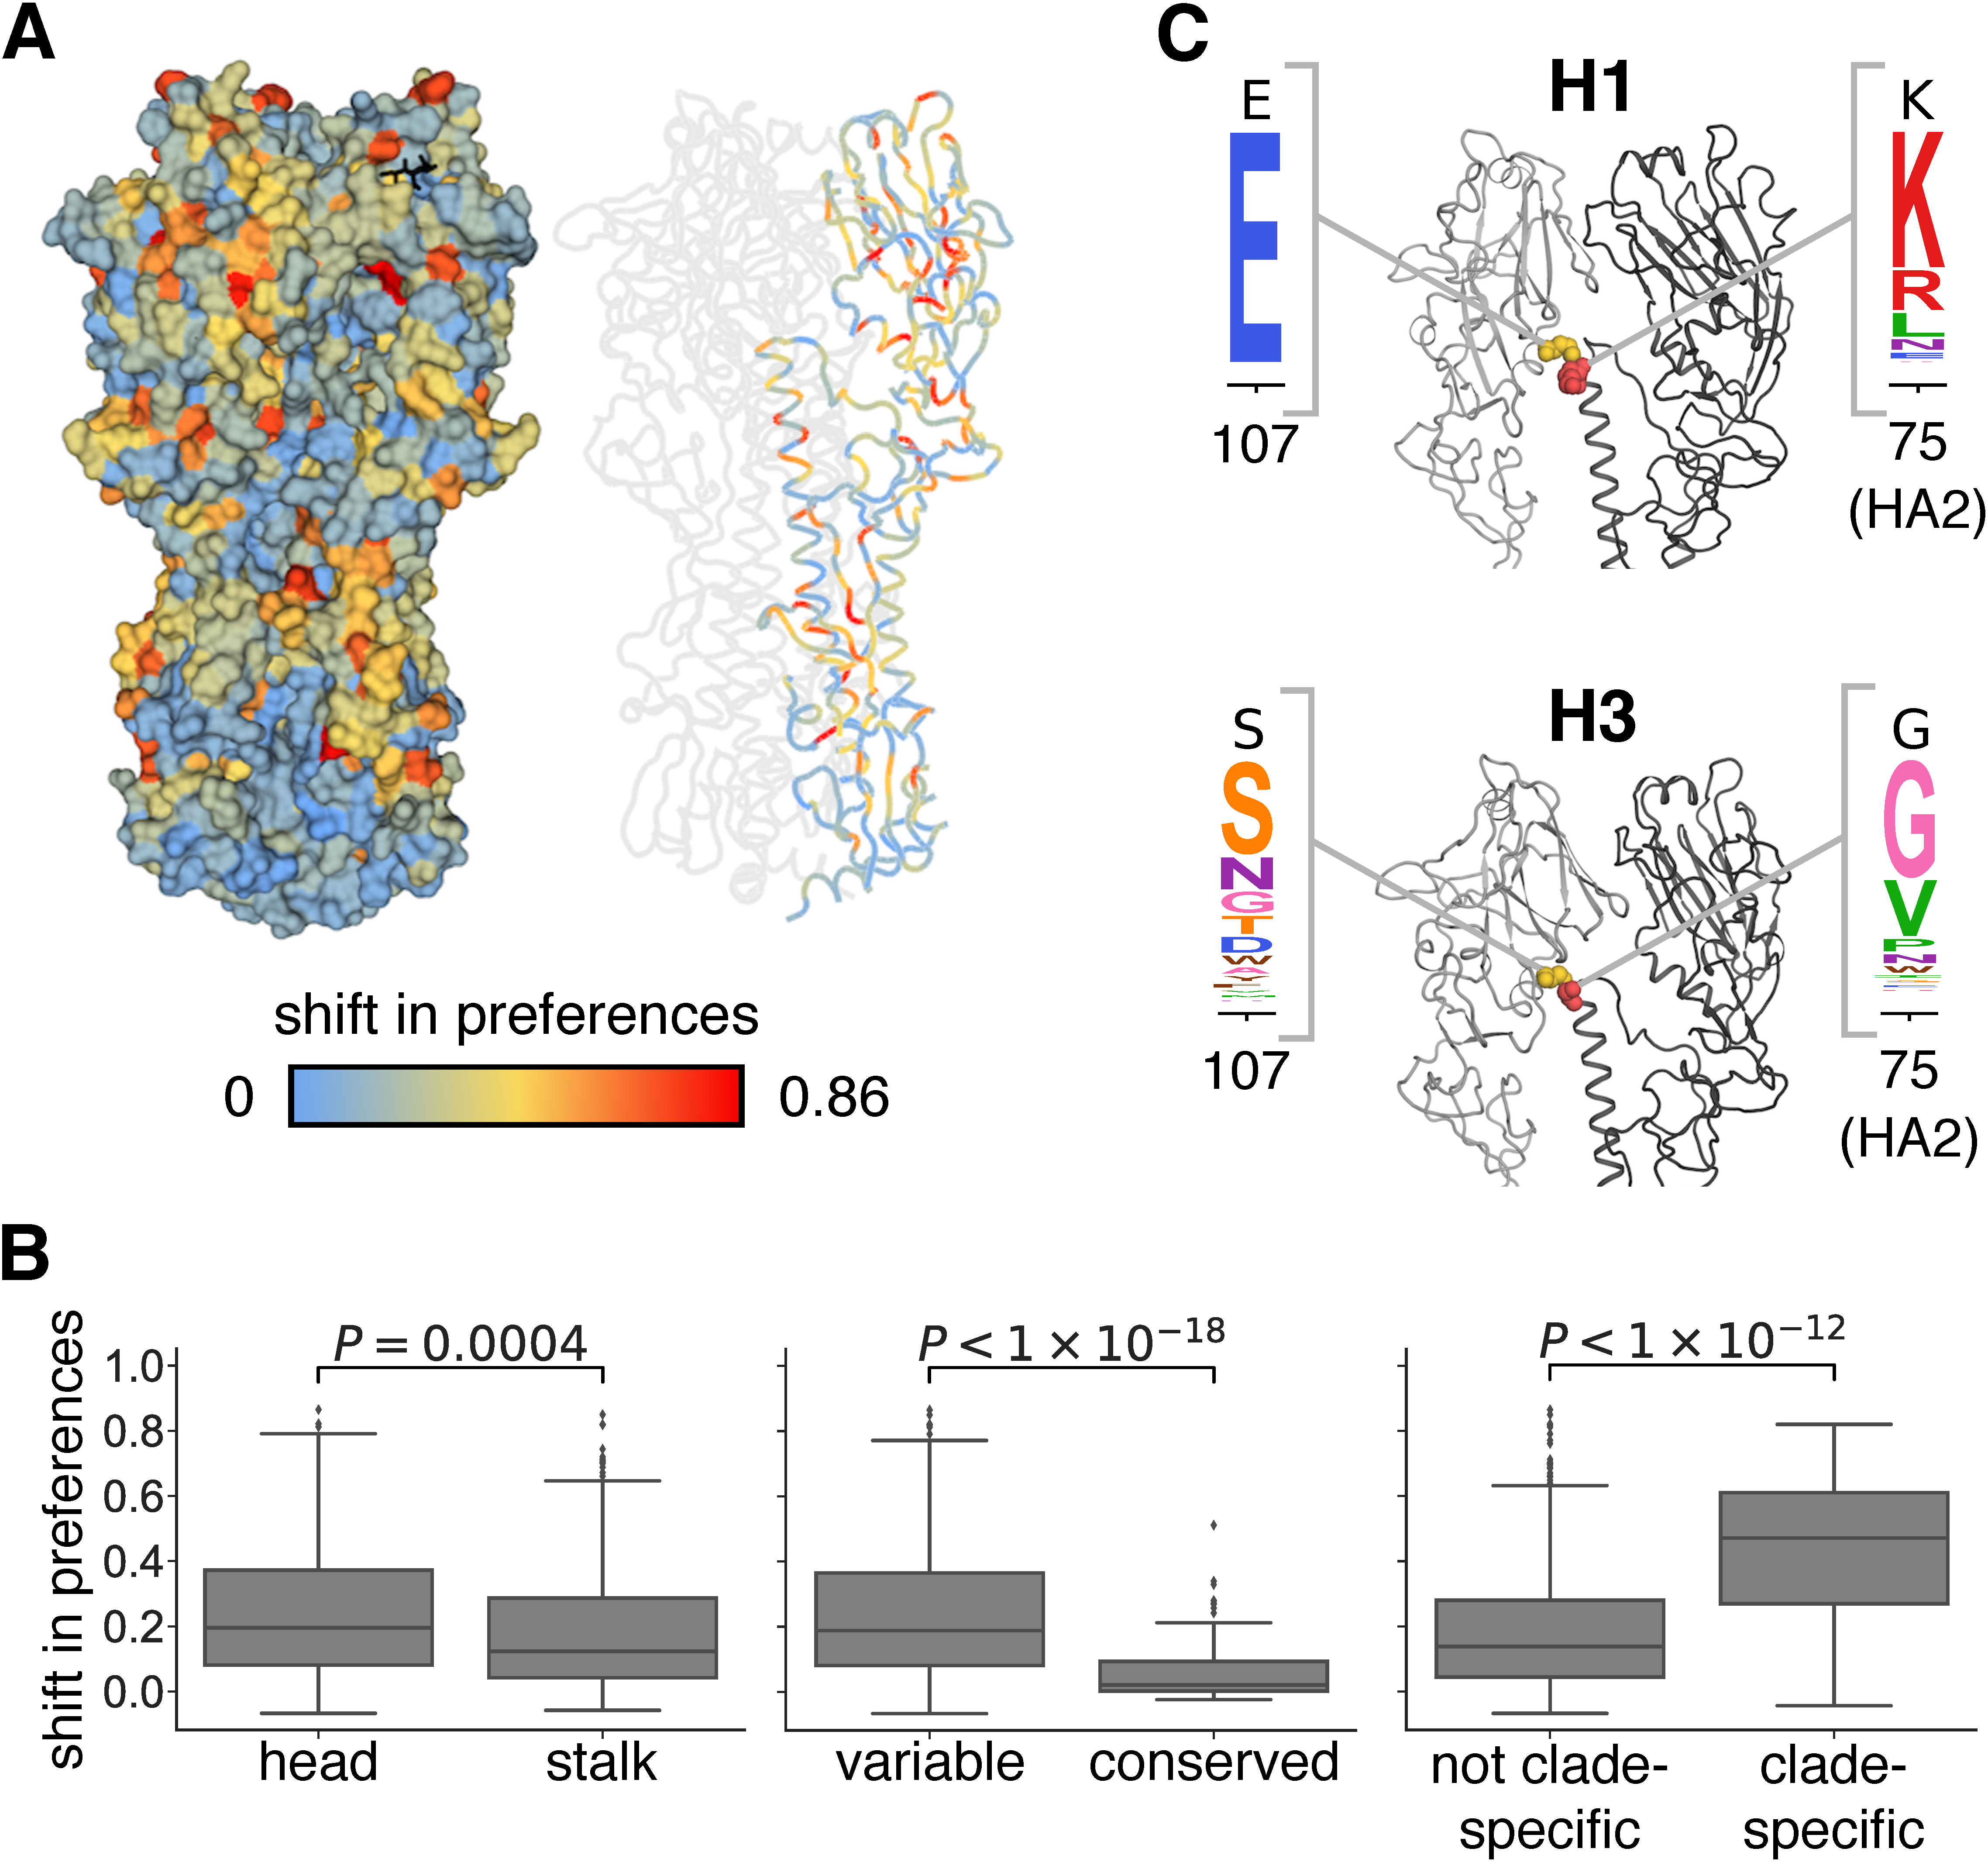
\includegraphics[width=16cm]{figs/RMSD_heatmap/RMSD_heatmap.pdf}
\caption{\label{fig:RMSD_heatmap}
{\bf Shifts in preferences mapped onto the structure of HA}
(A) The preference shifts as calculated by $RMSD_{corrected}$ between the two HA homologs is mapped onto the structure of HA (PDB 4O5N;~\cite{lee2014receptor}). 
The left structure shows the HA trimer, and the right structure colors one of the monomers. 
The sialic acid receptor is shown in black sticks.
Blue indicates small shifts in preference near zero, while red indicates large shifts in preference.
The top ten most shifted sites are shown in spheres on the monomer.
(B) The stalk domain was found to be significantly less shifted than the head domain (left plot).
Sites absolutely conserved all 18 HA subtypes were also found to be significantly less shifted than the remaining non-conserved sites (right plot).
(C) 
}
\end{figure*}

\section*{Discussion}
\label{sec:discussion}
We have measured the effect of all possible single amino-acid mutations to Perth/2009 H3 on viral growth in cell culture.



\matmethods{Please describe your materials and methods here. This can be more than one paragraph, and may contain subsections and equations as required. Authors should include a statement in the methods section describing how readers will be able to access the data in the paper. 

\subsection*{Subsection for Method}
Example text for subsection.
}

\showmatmethods{} % Display the Materials and Methods section

\acknow{Please include your acknowledgments here, set in a single paragraph. Please do not include any acknowledgments in the Supporting Information, or anywhere else in the manuscript.}

\showacknow{} % Display the acknowledgments section

% \pnasbreak splits and balances the columns before the references.
% Uncomment \pnasbreak to view the references in the PNAS-style
% If you see unexpected formatting errors, try commenting out \pnasbreak
% as it can run into problems with floats and footnotes on the final page.
%\pnasbreak

% Bibliography
\subsection*{References}
\bibliography{references}

% Supplementary material temporarily moved until AFTER everything else for initial submission

\onecolumn

\subsection*{Supporting Information (SI)}
\FloatBarrier

The main text of the paper must stand on its own without the SI. Refer to SI in the manuscript at an appropriate point in the text. Number supporting figures and tables starting with S1, S2, etc. Authors are limited to no more than 10 SI files, not including movie files. Authors who place detailed materials and methods in SI must provide sufficient detail in the main text methods to enable a reader to follow the logic of the procedures and results and also must reference the online methods. If a paper is fundamentally a study of a new method or technique, then the methods must be described completely in the main text. Because PNAS edits SI and composes it into a single PDF, authors must provide the following file formats only.

\subsubsection*{SI Text}

Supply Word, RTF, or LaTeX files (LaTeX files must be accompanied by a PDF with the same file name for visual reference).

\subsubsection*{SI Figures}

\begin{suppfigure}
\centerline{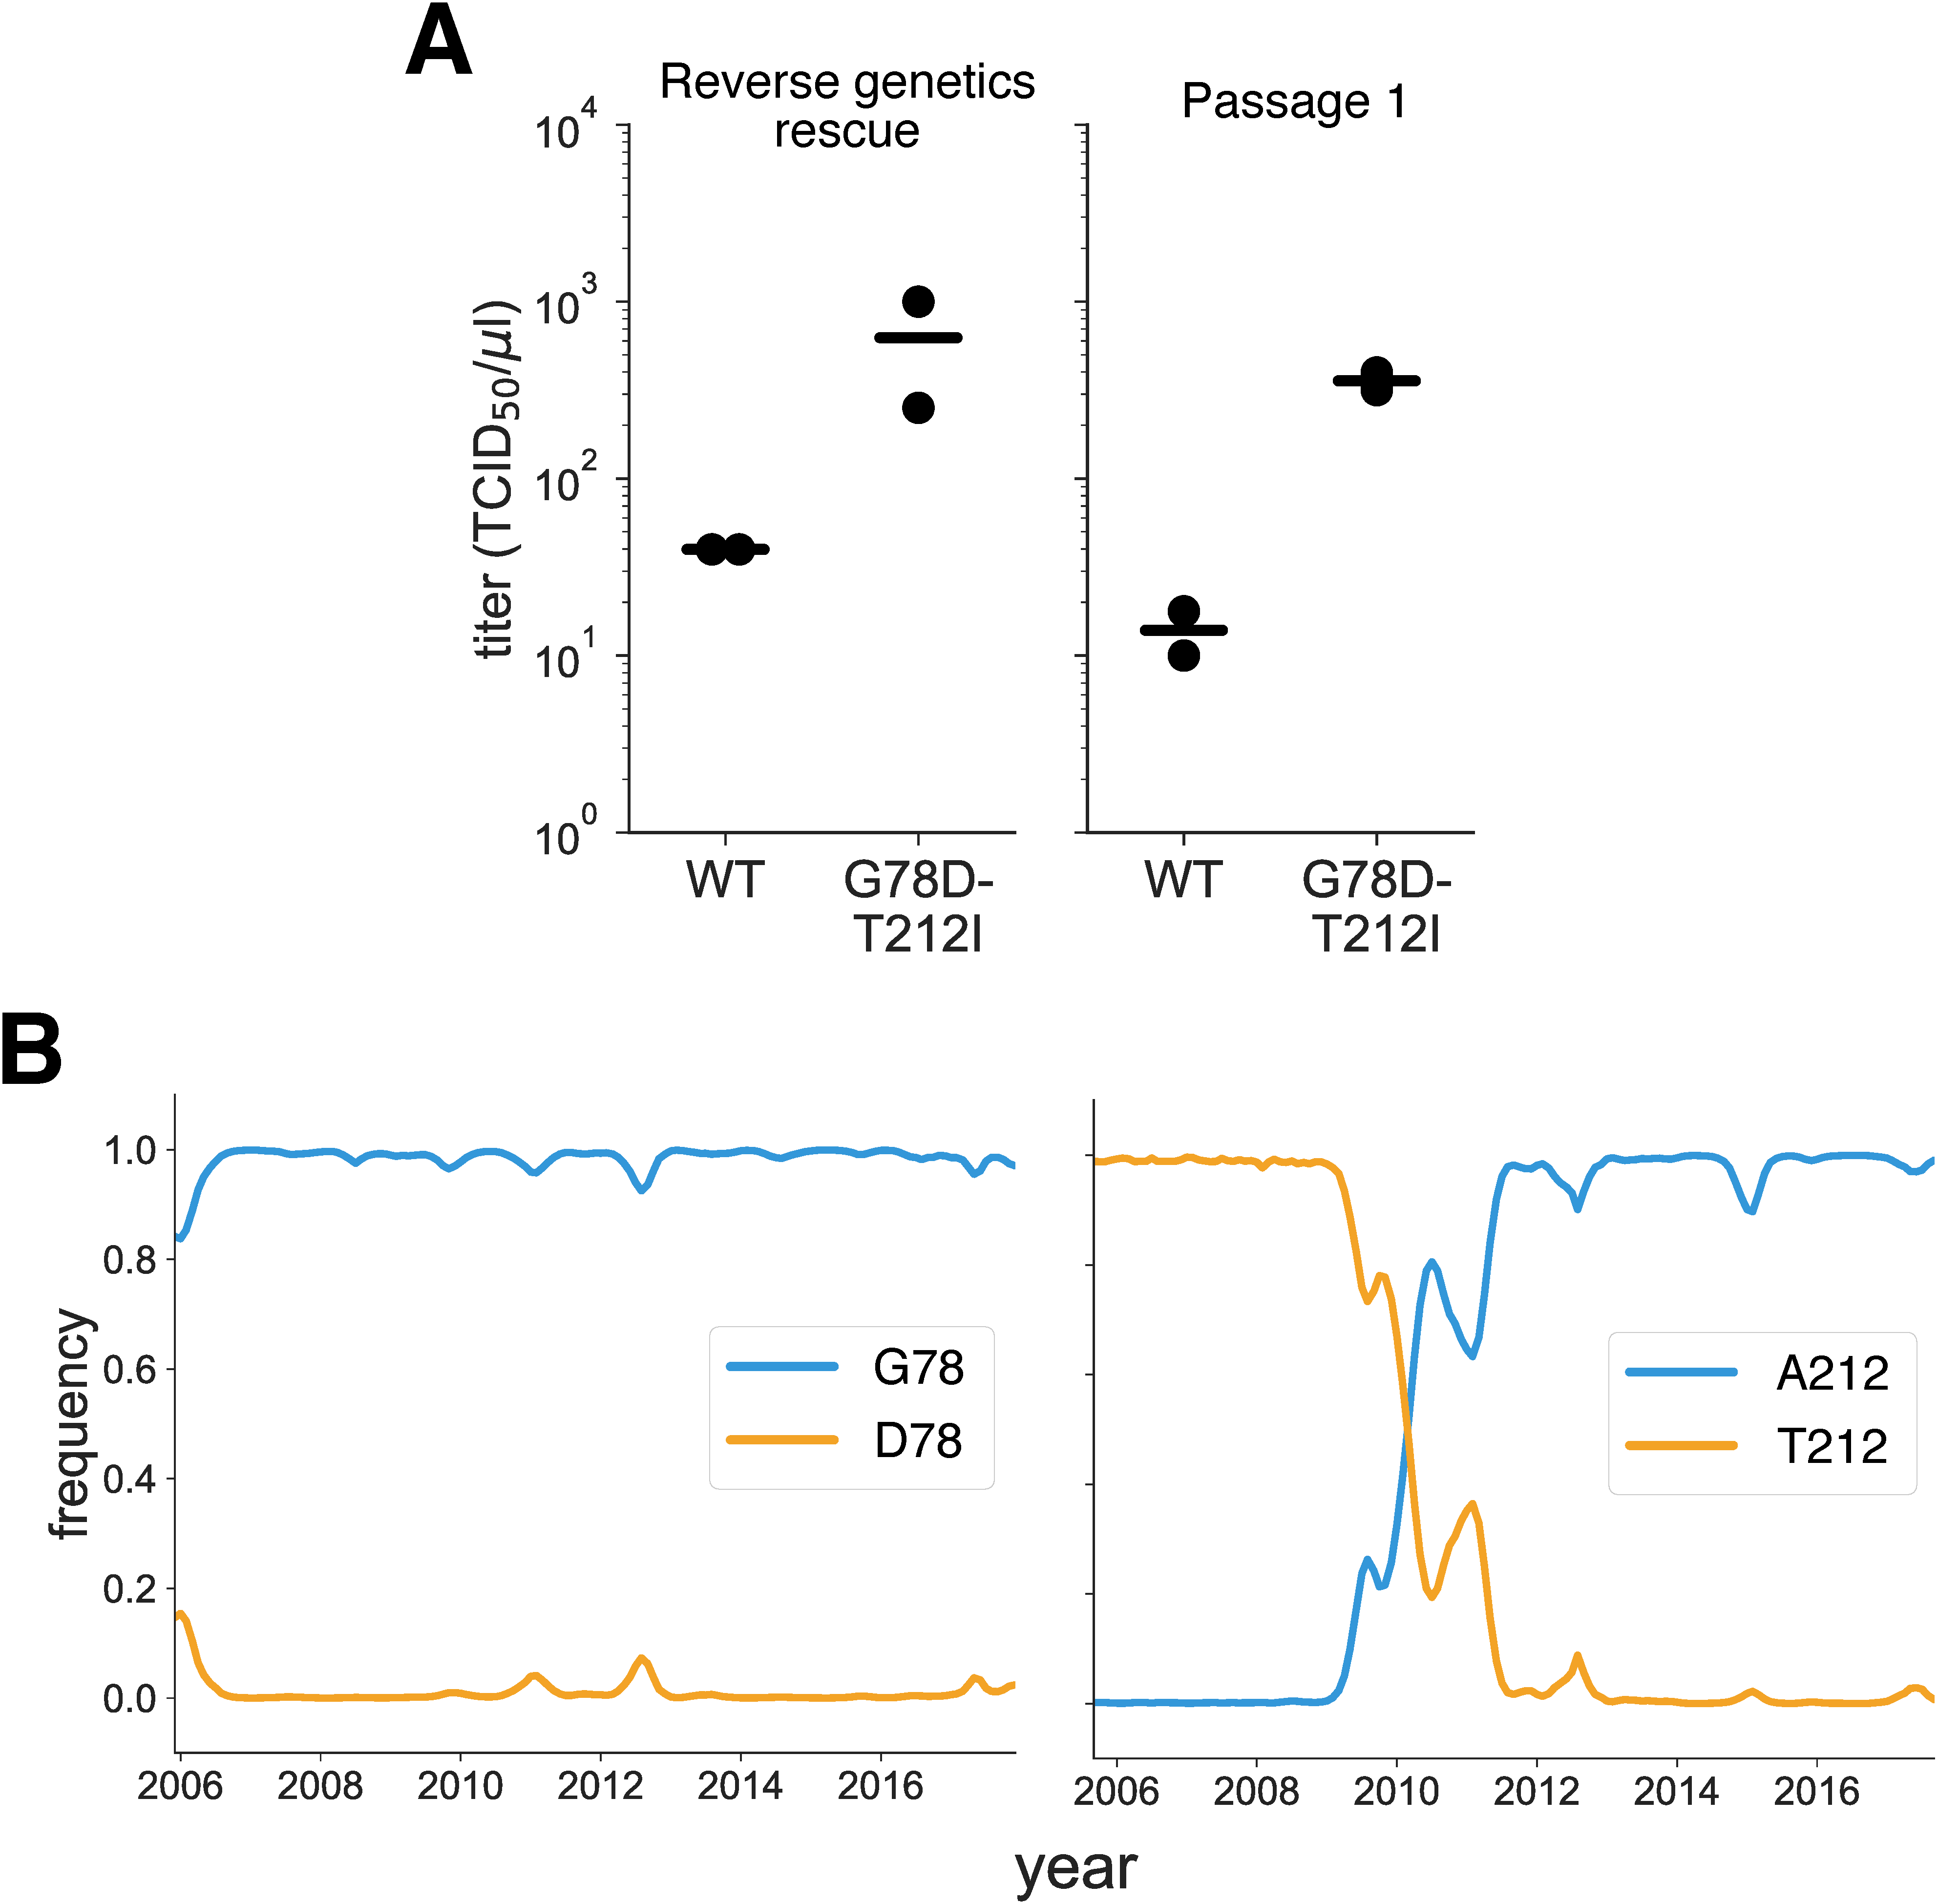
\includegraphics[width=0.5\textwidth]{figs/S01_G78D-T212I/G78D-T212I.pdf}}
\caption{\label{suppfig:Perth2009_mut}
{\bf Characterization of the G78D-T212I Perth/2009 HA variant.} 
(A) 
The G78D-T212I Perth/2009 HA variant supports better viral growth than the wildtype Perth/2009 HA.
Viruses were generated in duplicate by reverse genetics with the Perth/2009 NA and WSN internal genes, and passaged once at MOI = 0.01 in MDCK-SIAT1-TMPRSS2 cells.
The rescue and passage viral supernatants were collected at 72 hours post-transfection and 44 hours post-infection, respectively, and titered in MDCK-SIAT1-TMPRSS2 cells. 
The points mark each duplicate and the bar marks the mean.
(B)
The D78 variant remained at a low frequency in natural human H3N2 sequences over the past $~\sim$10 years.
The A212 variant rose to fixation in $~\sim$2011, replacing the T212 variant.
}
\end{suppfigure}

\subsubsection*{SI Tables}

Supply Word, RTF, or LaTeX files (LaTeX files must be accompanied by a PDF with the same file name for visual reference); include only one table per file. Do not use tabs or spaces to separate columns in Word tables.

\subsubsection*{SI Datasets} 

\begin{suppdata}
\caption{\label{suppdata:PerthHA}
Genbank file giving the full sequence of the bidirectional reverse-genetics plasmid pHW-Perth2009-HA-G78D-T212I, which encodes the wildtype HA sequence used in this study.
}
\end{suppdata}


\end{document}